\section{Settings}
The story is set in a extended version of the world presented in the movie which includes some elements taken from the books and some brand-new elements. In particular, we are going to talk about a race and some places that are never mentioned in the movie but we consider them as if they have been always existing.

%The story is set in an alternative universe, in a unspecified region of the Earth, where humans, magicians and djiins live.

\begin{itemize}
	\item \textbf{Humans}: the most common race. They live in contact with magicians.
	\item \textbf{Magicians}: humans with magic powers. They are less common than humans.
	\item \textbf{Djiins}: this race is so rare that it is considered like a legend. They are a long-living race, incredibly powerful and skilled in magic.
\end{itemize}

Everybody speaks the same language and lives according to the norms of civilized countries.

The atmosphere in the region resembles that of Japan in the early 1900s and it is organized in many different kingdoms.

Each king holds a court magician who helps him in the political and military affairs.

%Although the region seems safe and quiet, 

The Kingdom of Ingary is at war with the near Kingdom of Strangia. The war is fighted by soldiers and wizards.

%The current war is fighted by soldiers and wizards, called to duty by the court magicians on behalf of the kings.

\subsection{Flying castle (hub)}
It flies around the skies of Ingary. There is a magic door that lets you reach different places:
\begin{itemize}
	\item \textit{Green}: used to get out of the flying castle
	\item \textit{Red}: linked with Kingsbury
	\item \textit{Light blue}: linked with Dynamia
	\item \textit{Black}: linked with the past
\end{itemize}
\begin{figure}[H]
  \centering
  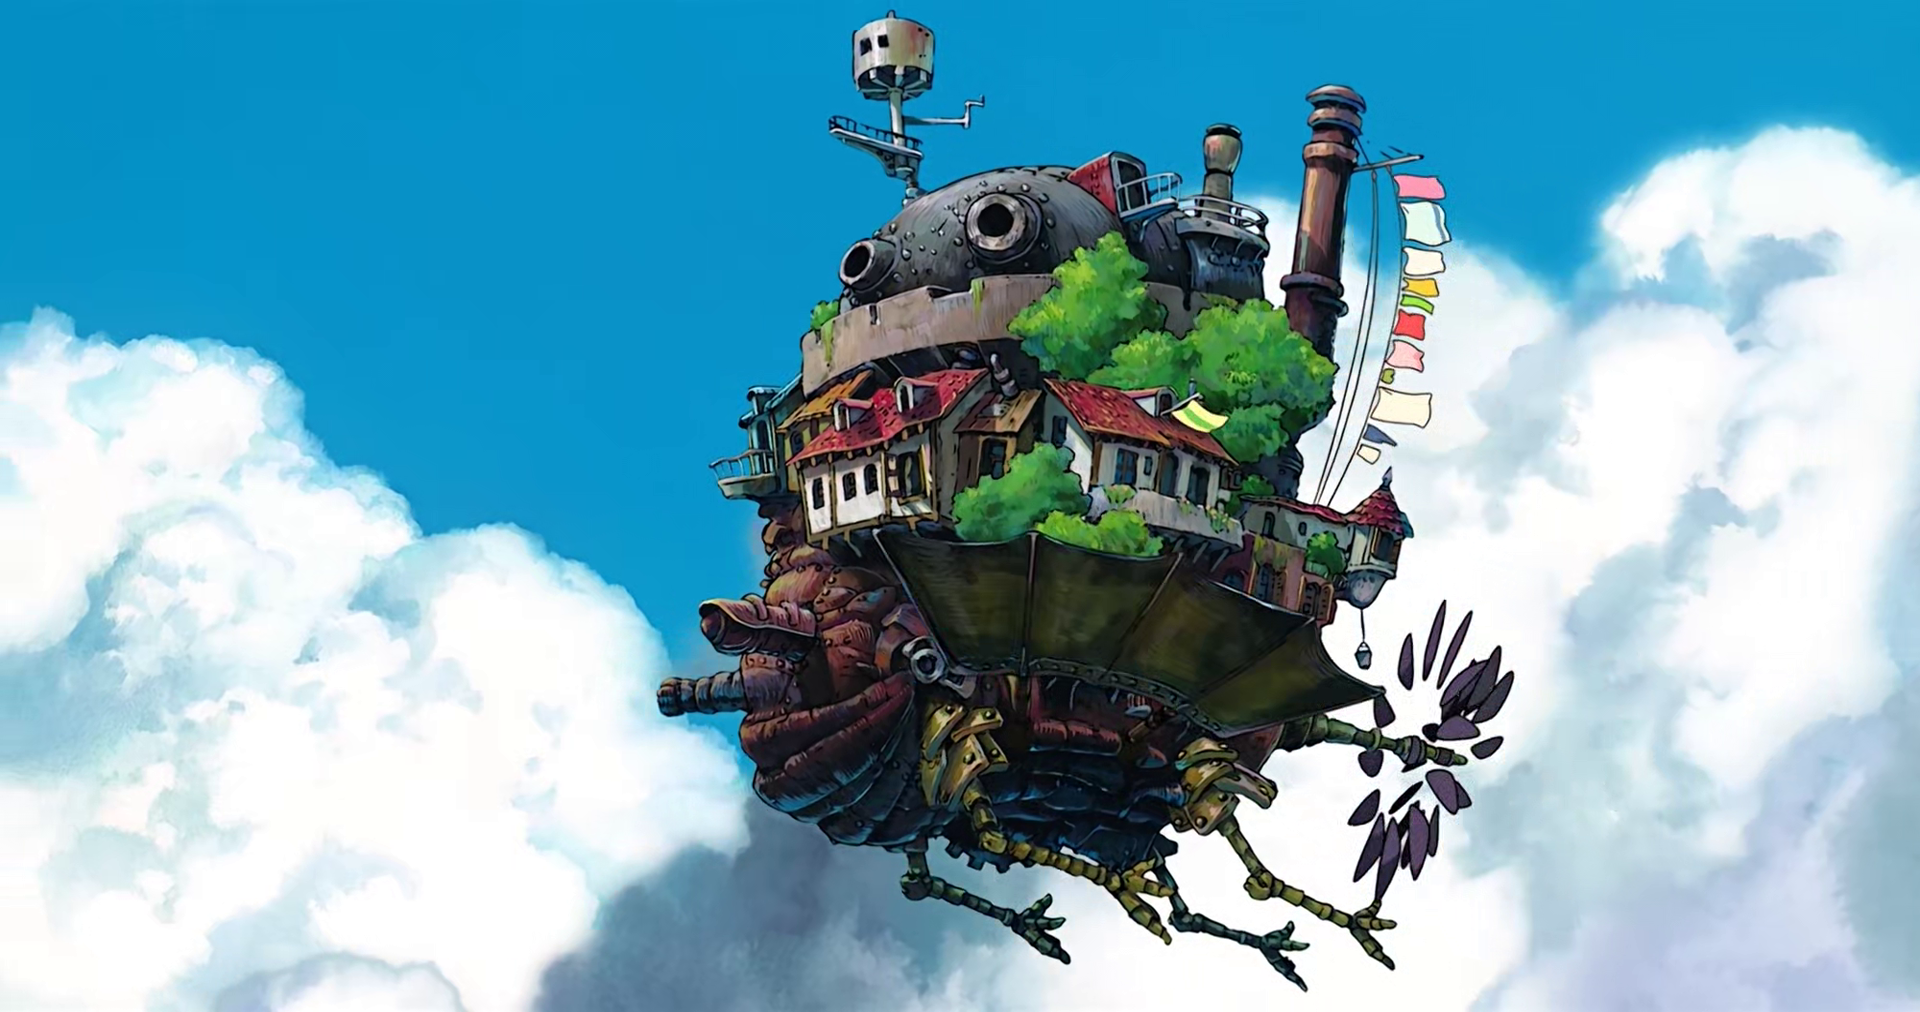
\includegraphics[width=12cm]{../Images/Locations/flyingCastle}
  \caption{Flying castle, movie version}
\end{figure}

\subsection{Kingsbury}
The capital of the Kingdom of Ingary. It is a rich city positioned on a river in a wide plain.
\begin{figure}[H]
  \centering
  
\includegraphics[width=12cm]{../Images/Locations/kingsbury}
  \caption{Kingsbury, movie version}
\end{figure}

\subsection{Kingsbury under attack}
During the attack of the demons from Strangia, the capital is in chaos and many buildings are damaged or burning, but the castle is safe.
\begin{figure}[H]
  \centering
  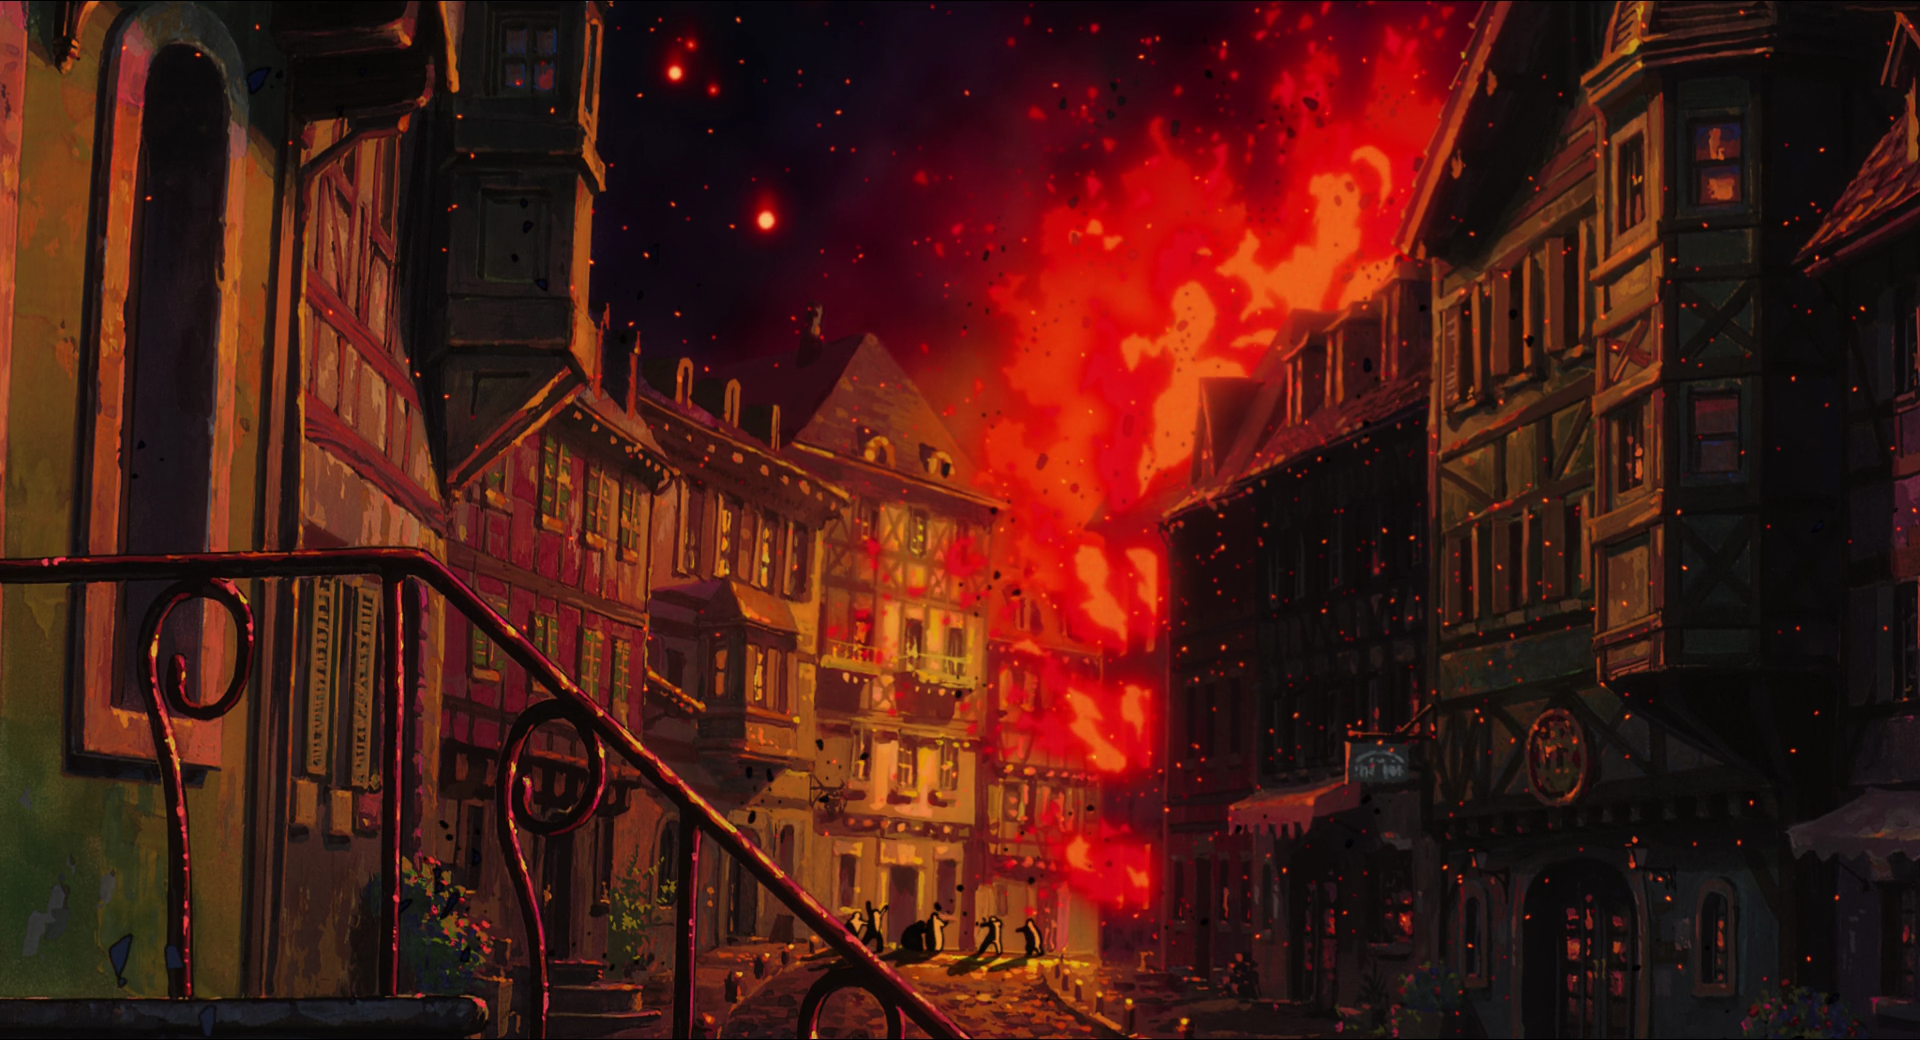
\includegraphics[width=12cm]{../Images/Locations/kingsburyUnderAttack}
  \caption{Reference image for Kingsbury under attack from the movie}
\end{figure}

\subsection{Dynamia}
The capital of the Kingdom of Strangia. It is built on a lagoon and its streets are canals.
\begin{figure}[H]
  \centering
  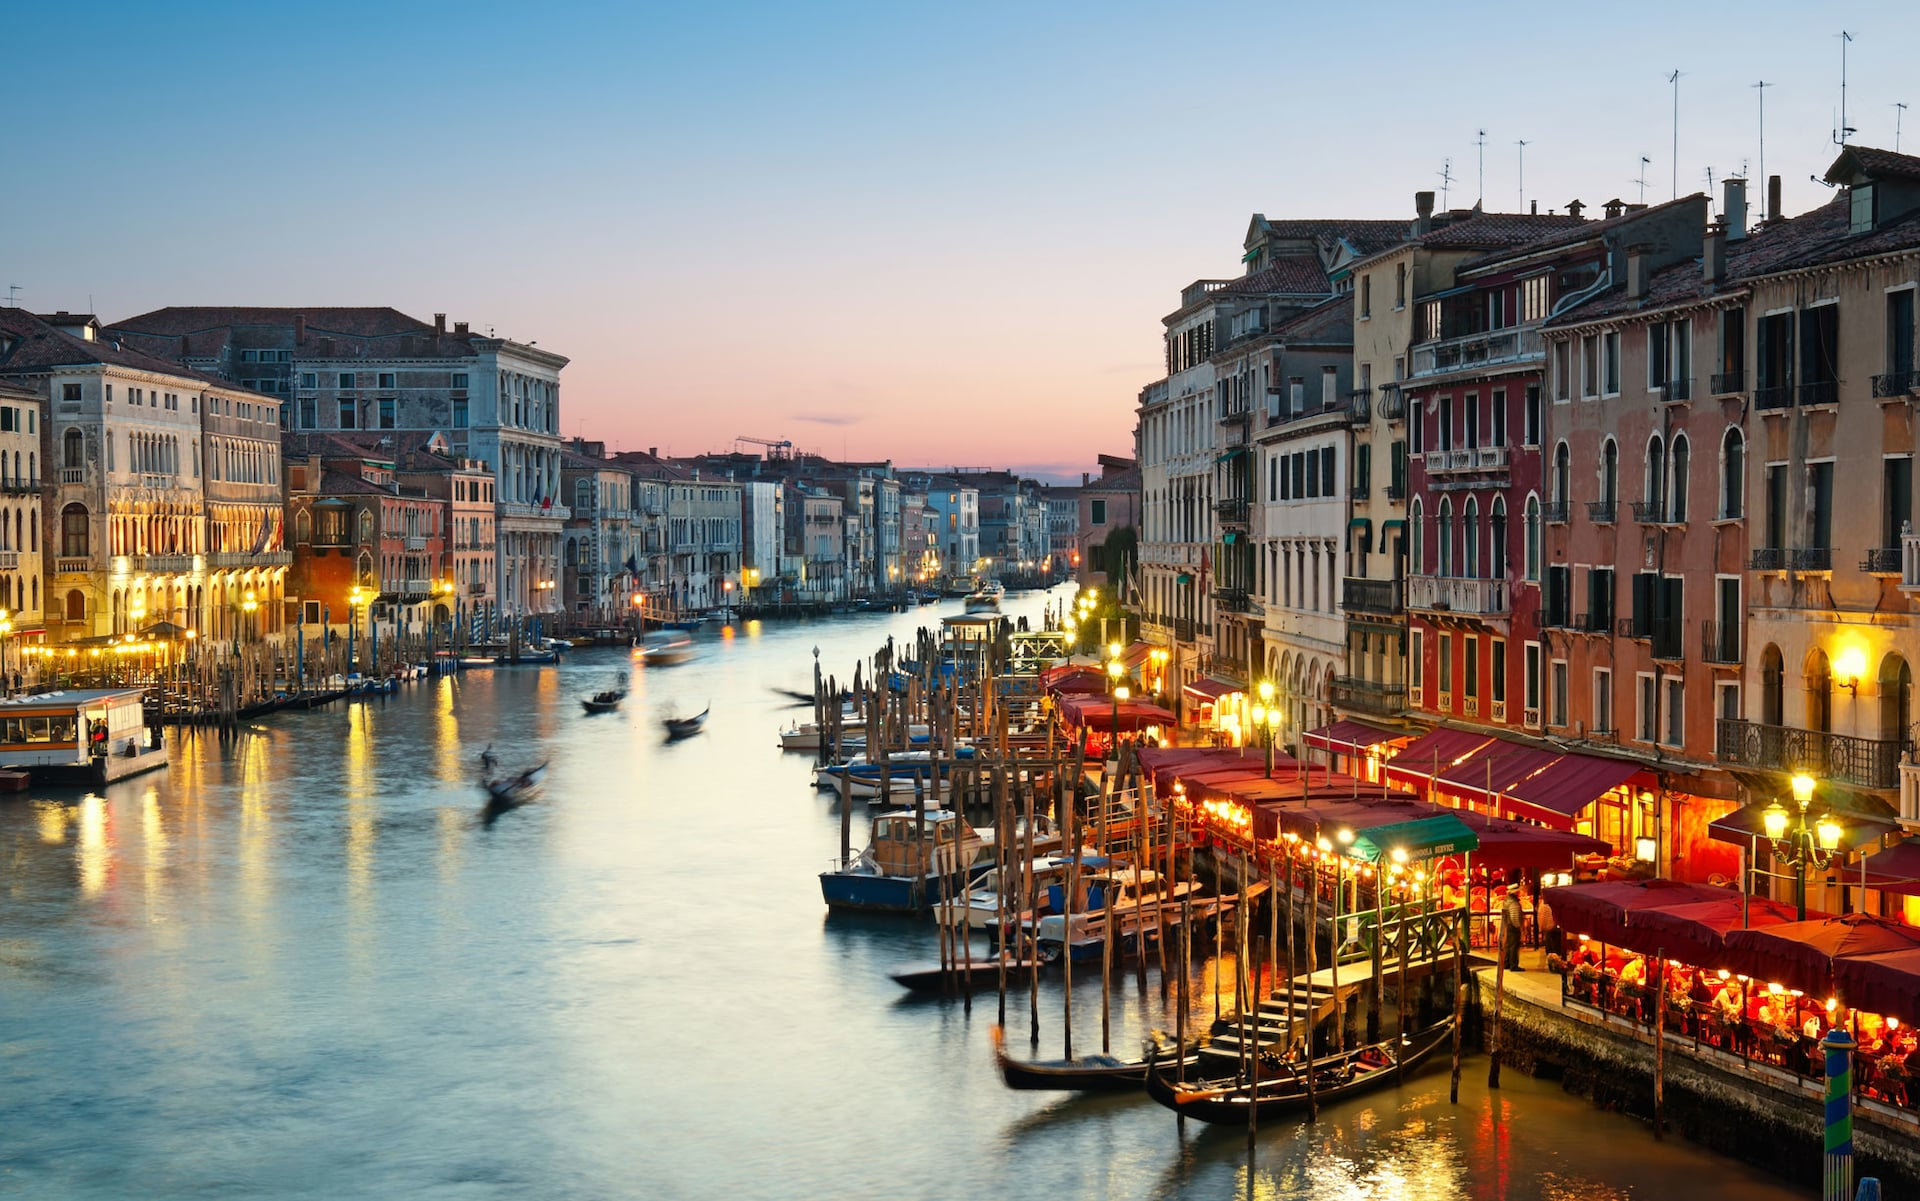
\includegraphics[width=12cm]{../Images/Locations/dynamia}
  \caption{Reference image for Dynamia}
\end{figure}

\subsection{Southern deser}
A big uninhabited region. According to a legend, an old powerful djinn lives here.
\begin{figure}[H]
  \centering
  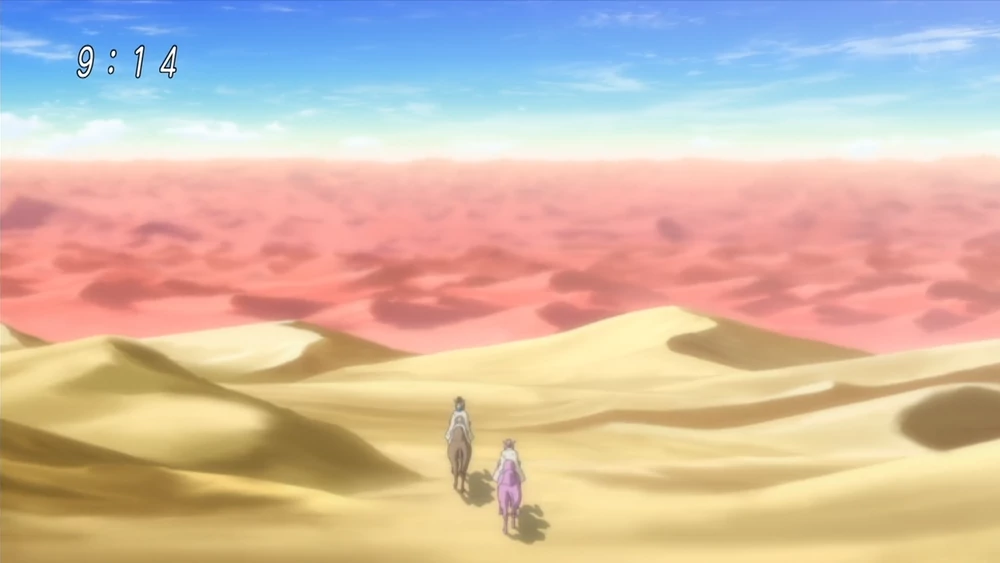
\includegraphics[width=12cm]{../Images/Locations/southernDesert}
  \caption{Reference image for the Southern desert}
\end{figure}

\subsection{Spirits real}
A magical parallel dimension where spirits of dead people live. There are no artificial things, everything is crafted by nature and magic. Only djinns are enough powerful to create portals to get there. Even the most powerful magicians can not enter into the spirits realm using only their own skills.
\begin{figure}[H]
  \centering
  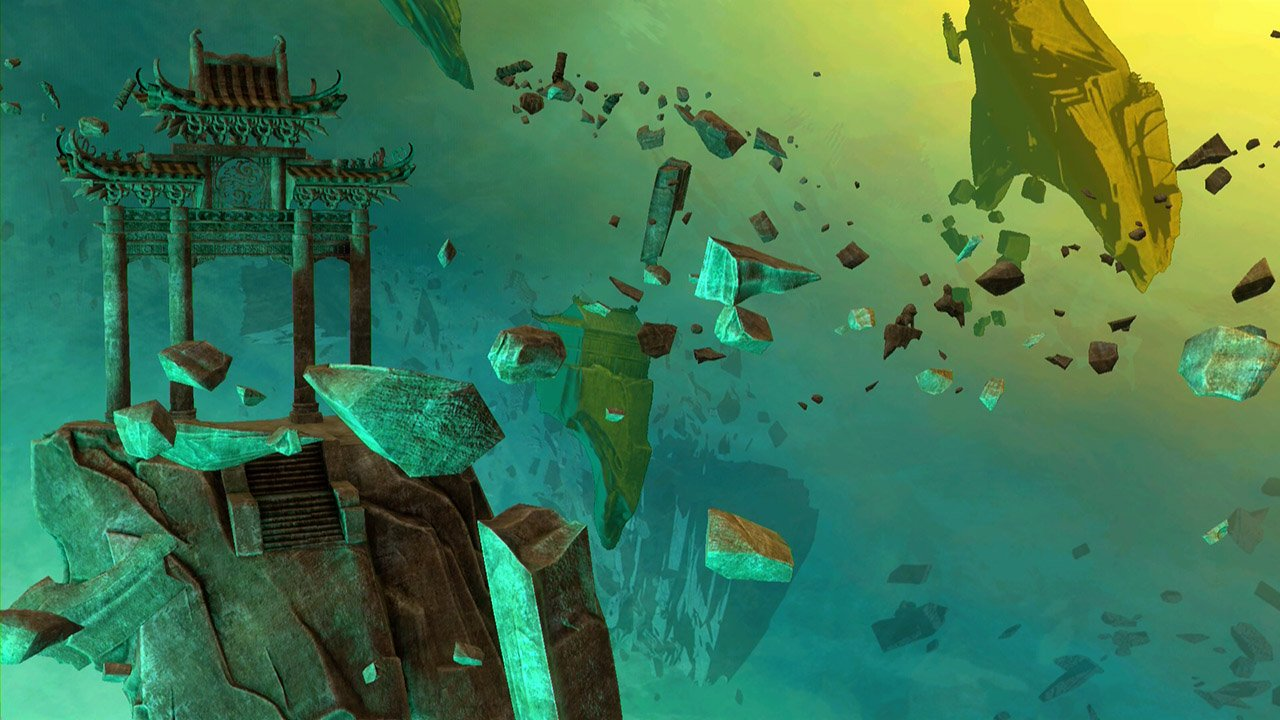
\includegraphics[width=12cm]{../Images/Locations/spiritsRealm}
  \caption{Reference image for the spirits realm}
\end{figure}

\subsection{Kazan island}
A volcanic island away from the coasts of the continent where Mizar has hidden her heart.
\begin{figure}[H]
  \centering
  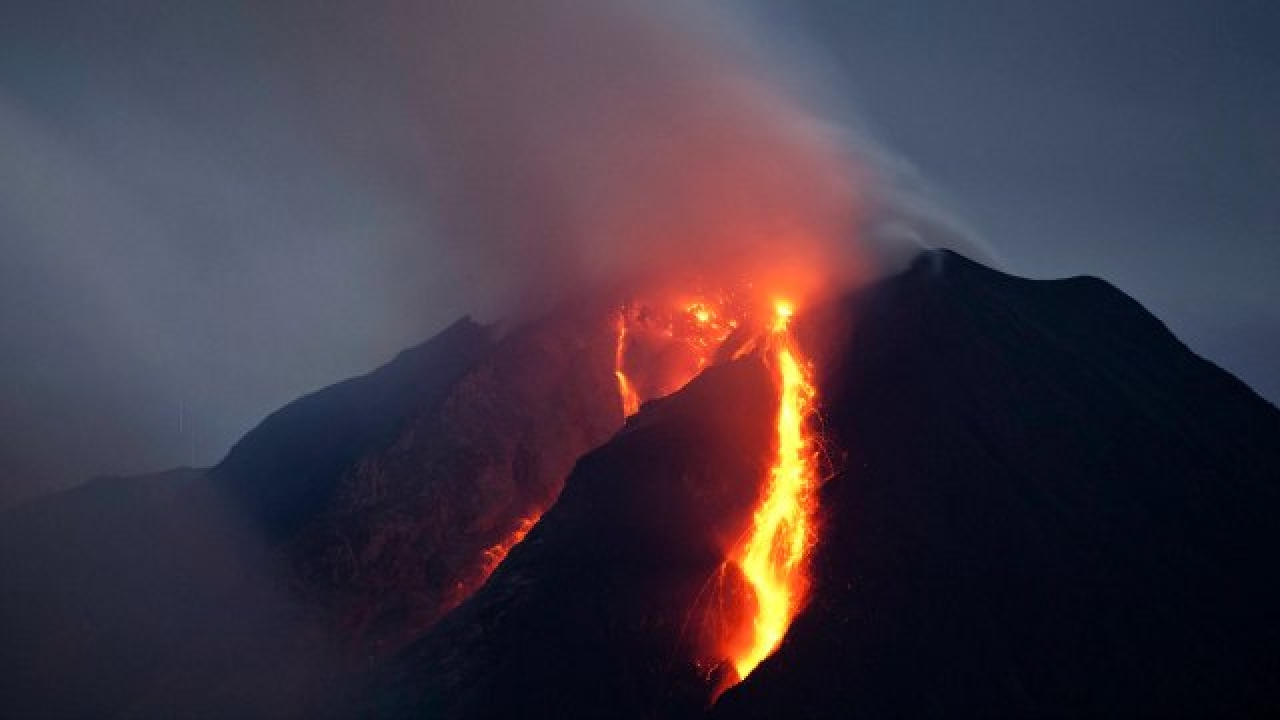
\includegraphics[width=12cm]{../Images/Locations/kazanIsland}
  \caption{Reference image for Kazan island}
\end{figure}

%\item \textit{Kazan island}: a volcanic island away from the coasts of the continent. In the depths of the dormant volcano Mizar has hidden her heart.
For more reference images: \url{http://wastelandsteam.altervista.org/category/locations/}\\
Password: \textit{gld18}
